\documentclass[a4paper,fleqn]{article} %Options in documentclass should be set to a4paper and fleqn.
\usepackage{modsim}
\usepackage{times}
\usepackage{natbib} %The three packages modsim, times and natbib are required.
\usepackage{amsmath, amssymb, amsthm} %Also recommend the standard AMS LaTeX maths packages.

\pagestyle{MODSIMheadings} %Calling the MODSIM Headings format
\MODSIMhead{F. Chan and L. Pauwels, Unit roots and structural breaks in panel...} %This is the content of the headings in all pages (except the first page). The format should be author, title of paper. If the title is too long, then use ... at the end. If more than two authors, then please use the "et al." format with et al. in italic, for example A. Author {\it et al.}, Title of the paper.

% Define any other command or required packages below:
%%%%%%%%%%%%%%%%%%%%%%%%%%%%%%%%%%%%%%%%%%%%%%%%%%%%%%%%%%%%%%%%%%%%%%%%%%%%%%%%%%%%%%%%%%%%%%%%%%%%%%%%%%%
\usepackage{rotating}
\usepackage{amsbsy,enumerate}
\usepackage{graphicx}
\usepackage{ccaption}
\newcommand{\ve}{\varepsilon}
\newcommand{\sigmah}{\hat{\sigma}}
\newcommand{\sigmab}{\bar{\sigma}}
\newcommand{\R}{\mathbb{R}}
\newcommand{\Z}{\mathbb{Z}}
\newcommand{\E}{\mathbb{E}}
\newcommand{\Tbar}{\bar{T}}
\newcommand{\Thetabf}{\mathbf{\Theta}}
\newcommand{\Xbf}{\mathbf{X}}
\newcommand{\xbf}{\mathbf{x}}
\newcommand{\Ybf}{\mathbf{Y}}
\newcommand{\ybf}{\mathbf{y}}
\newcommand{\Ubf}{\mathbf{U}}
\newcommand{\Fbf}{\mathbf{F}}
\newcommand{\fbf}{\mathbf{f}}
\newcommand{\Pbf}{\mathbf{P}}
\newcommand{\Pbfbar}{\bar{\mathbf{P}}}
\newcommand{\Sb}{\bar{S}^{\nu}}
\newcommand{\Snuib}{\tilde{S}^\nu _i}
\newcommand{\Snui}{S^\nu _i}
\newcommand{\sigmanui}{\sigma ^\nu_i}
\newtheorem{lemma}{Lemma}
\newtheorem{corollary}{Corollary}
\newtheorem{assumption}{Assumption}
\newtheorem{theorem}{Theorem}
\newtheorem{remark}{Remark}
\newtheorem{definition}{Definition}
\newtheorem{cce}{Assumption CCE}
\newtheorem{proposition}{Proposition}
%% The next four lines create the correct format for Figure and Table captions. They require the package "ccaption".
\makeatletter
\renewcommand{\fnum@figure}[1]{\textbf{\figurename~\thefigure}. }
\renewcommand{\fnum@table}[1]{\textbf{\tablename~\thetable}. }
\makeatother

%%%%%%%%%%%%%%%%%%%%%%%%%%%%%%%%%%%%%%%%%%%%%%%%%%%%%%%%%%%%%%%%%%%%%%%%%%%%%%%%%%%%%%%%%%%%%%%%%%%%%%%%%%%

\begin{document}
% Defining Front matter.

\title{Unit Roots and Structural Breaks in Panels: Does the Model Specification Matter?}

\author{F. Chan \address[A1]{\it{School of Economics and Finance, Curtin University, GPO BOX U1987, Perth, Western Australia, 6845}}, \underline{L. Pauwels} \address[A2]{\it Discipline of Econometrics and Business Statistics, University of Sydney, Australia}} %underline the name of the presenting author. Use \addressmark[name-of-addressmark] after the name of an author who share the same affiliation (see modsim.tex for an example).

\email{L.Pauwels@econ.usyd.edu.au} %Email address of the presenting author only.

\date{June 2017}

%Keywords should be separated by commas and listed in Sentence case (first keyword with capital first letter and remaining keywords in lower case).
\begin{keyword}
Structural change, unit roots, cross sectionally dependent errors, heterogeneous panels, Monte Carlo, Univariate time series
\end{keyword}

\begin{abstract}
	Although the impacts of structural instability on testing for unit root have been studied extensively for univariate time series, such impacts on panel data unit root tests are still relatively unknown. A major issue is the choice of model in accommodating different types of break (instability) prior to testing for unit root. Specifically, researchers must specify a potential break in the intercept, the trend or both before testing for unit root. Model misspecification has been known to have a great impact on the test performance in the univariate case, especially when the selected model fails to accommodate a break in the trend. However, the impact of model misspecification on testing for unit root is still unknown for panel data. \par
	This paper has two objectives: (i) it proposes a new test for unit root in the presence of structural instability for panel data. The test allows the intercepts, the trend coefficients or both to change at different date for different individuals. Under some mild assumptions, the test statistics is shown to be asymptotically normal which greatly facilitates valid inferences. (ii) Using the proposed test, this paper provides a systematic study on the impact of structural instability on testing for unit root using Monte Carlo Simulation. Specifically, the impact of model misspecification on the size and the power of the proposed test is discussed in details.\par
	Although the test performs reasonably well when the models are correctly specified, Monte Carlo results show that failure to accommodate a break in the trend coefficients can seriously distort the size and the power of the proposed test. In fact, the power of the test decreases when individuals experience a break in the trend coefficients even when the model is correctly specified. This is consistent with the results for univariate time series.
\end{abstract} %Abstract should NOT extend beyond the first page.

\maketitle

\section{INTRODUCTION}

In the time-series literature, the presence of intercept and/or slope structural change has altered the perception of unit root testing as structural breaks lead very often to the under-rejection of the null hypothesis. See for example the seminal work by \citeauthor{Perron:1989} (\citeyear{Perron:1989}, \citeyear{Perron:1990}), \citet{Perron:1992}. Perron's test was subsequently modified for the case of unknown (determined endogenously) breakpoint by \citet{Zivot:1992} who provided a minimum t-statistic testing the null of a unit root with no breaks against the alternative of one unknown break. \citet{Lumsdaine:1997} extended \citet{Zivot:1992} for two breakpoints. \citet{Lee:2003} have recently provided a unit root test of the null hypothesis of a unit root with two unknown breaks against the alternative of trend stationary data with two unknown breaks.

In the \citet{Zivot:1992} and \citet{Lumsdaine:1997} [henceforth ZA and LP respectively], the null hypothesis of a unit root is tested for each variable of concern against the alternative of unknown structural break(s). The rejection of the null of the ZA and LP tests does not necessarily imply stationarity with structural breaks unlike the \citet{Perron:1989} test.  The alternative indicate that there are structural breaks and still includes the possibility of unit roots with breaks. This ambiguity might be exacerbated as the magnitude of the break increases as pointed out by \citet{Nunes:1997}, \citet{Vogelsang:1998}, and \citet{Lee:2001}. The \citet{Perron:1989} test on the other hand allows for potential breaks under both the null and the alternative hypotheses. Under the alternative the variables are stationary with an exogenous structural break. More recently, \citet{Lee:2003} address some of the limitations \citet{Perron:1989}, \citet{Zivot:1992} and \citet{Lumsdaine:1997} techniques, by providing a minimum LM test unit root test for the null of a unit root with two unknown breakpoints against an unambiguous alternative of trend stationarity with two unknown breaks.

An issue which has received little attention in this empirical literature is whether selecting the appropriate type of break matters for the size and power of unit root tests in panel data models as $N$ grows large? This problem was first pointed out by \citet{Lumsdaine:1997} in the time-series literature. So far, most applications of these tests have relied on observing the data to determine the type of breaks. \citet{Perron:1989} distinguishes three types of additive outlier models (level shift, slope change or both) and two innovative outlier models (level shift and both).  As highlighted by \citet{Zivot:1992} in comparing exogenous versus endogenous break date determination, relying on observing data and subsequently running the statistical tests may be methodologically improper. As an empirical example, \citet{Perron:1989} tested for unit root with an exogenous break on the Nelson-Plosser macroeconomic data series. \citet{Perron:1989} relied primarily on descriptive statistics and graphs in order to discriminate between the use of one model or the other. \citet{Zivot:1992}, \citet{Lumsdaine:1997} and \citet{Lee:2003}, all have relied on Perron's choice of model in the Nelson-Plosser data series to run their specific tests and evaluate their performance. Though the literature has indicated that ignoring the presence of breaks when testing for unit roots affected tests, it has yet to be assessed whether right or wrong model selection ultimately affect the power and size of unit root test. \par

This paper extend the recent \citet{KimPerron:2009} methodology in the panel data context in order to assess whether model specification matters for unit root tests. This methodology provides the advantage that (a) it allows for a break both under the null and the alternative hypothesis and (b) their testing procedure is robust to the case where no break occurs under the null hypothesis of a unit root. This robustness is ensured by using pre-testing method for a break valid whether the noise component is integrated or stationary developed by \citet{PerronYabu:2009}. Once \citet{KimPerron:2009} methodology is extended, a series of Monte Carlo experiments are conducted to determine whether model specification has an impact on panel data unit root testing in panel data. Section 2 presents a review of the panel literature on unit root tests with breaks. Section 3 extends the \citet{KimPerron:2009} tests for panel data. Selected Monte Carlo simulations results will be presented in Section 4 and section 5 will contain some concluding remarks.


\section{TESTING FOR UNIT ROOTS WITH BREAKS IN PANEL DATA}

The panel data literature has witnessed recently an upsurge of interest in extending non-stationary procedures typical in time-series to the panel data models with the presence of single or multiple structural breaks, sometimes allowing for different individuals to have breaks at different point in time and for breaks to occur at unknown point of time. \citet{Carrion:2002} proposed a panel data version of the \citet{Perron:1989} test and are among the first to consider testing the null hypothesis of a unit root against the alternative of structural break in panel data. They extend and build their test based on the panel data unit root test by \citet{Harris:1999},  allowing for a level shift in the deterministic part. \citet{Harris:1999} rely on limiting distributions based on $N$, the number of individuals and a fixed $T$, which \citet{Carrion:2002} endorse in the construction of their procedure. The test relies on the assumption that each individual is independent of any other.

Subsequent papers have focused on the presence of both single and multiple structural breaks in panels in order to overcome the bias and the potential misspecification that can arise when testing for unit roots. \citet{Im:2005} derive a unit root LM test with one structural break in the trend, but the slope of the time trend does not change. They show that the panel LM unit-root test is not only robust to the presence of structural shifts, but is more powerful than the popular \citet{Im:2003} (IPS) test when there is no break. Their simulation results show that there is no serious size distortions as well as no significant power loss when one controls for non-existent shift.

\citet{Carrion:2005} develop KPSS tests within a multiple break framework at different unknown dates, allowing for different number of breaks for each individual. These are extensions of the panel test developed by \citet{Hadri:2000} but with the presence of structural changes. \citet{Carrion:2005} use \citet{Bai:1998} to detect the dates and number of structural changes in each time-series in order to test for the null of a panel unit root. The individual KPSS tests allowing for structural breaks are averaged in a similar fashion to \citet{Im:2003} and \citet{ChanManciniPauwels:2009} for example. Their approach is general enough to cover the cases of structural breaks in the mean and/or the trend but without specifying the break type in the model.

\citet{BaiCarrion:2004} also develop a test for the null hypothesis of a unit root with multiple structural breaks and rely on a similar setting as in \citet{Carrion:2002} and \citet{Carrion:2005}. Their main contribution, however, is to overcome the assumption of cross sectional independence made in \citet{Carrion:2005}. They model the dependencies in terms of the common factors analysis proposed by \citeauthor{Bai:2002} (\citeyear{Bai:2002}, \citeyear{Bai:2004}), which aims to distinguish between co-movements and idiosyncratic shocks affecting individual time series. Extracting the co-movements between the individual series allow to focus on individual specific shocks.

\section{A NEW TEST}
This section extends the recent \citet{KimPerron:2009} methodology in the panel data context. Consider the following Data Generating Processes (DGPs) for three different scenarios, namely Models A, B and C:

\begin{equation}
	y_{it}=x'_{it} \theta_{1i} + z(T_1)'_{it} \theta_{2i} + u_{it} \qquad i=1,\dots,N \quad t=1,\dots,T \label{eq:model}
\end{equation}
with
\[
u_{it} \sim NIID(0,1)
\]
where $x_{it}=(1,t,y_{it-1})'$ and $\theta_{1i}=(\alpha_i,\gamma_i, \rho_i)'$ and
\begin{displaymath}
z(T_{1})'_{it} = \left\{ \begin{array}{cc}
DC_{it}  &\textrm{for model A}\\
DT_{it}  &\textrm{for model B}\\
(DC_{it}, DT_{it})' & \textrm{for model C},
\end{array}  \right.
\end{displaymath}
\begin{displaymath}
\theta_{2i} = \left\{ \begin{array}{cc}
d\alpha_i  &\textrm{for model A}\\
d\gamma_i  &\textrm{for model B}\\
(d\alpha_{i}, d\gamma_{i})' & \textrm{for model C}
\end{array}  \right.
\end{displaymath}
$DC_{it}=DT_{it}=0$, if $t<T_1$ for some $i \in \{1, \ldots, N\}$ and $DC_{it}=1$, $DT_{it}=t-T_1$, if $t>T_1$ for some $j \in \{1, \ldots, N\}$, and $j \neq i$.
/bin/bash: ibtex: command not found
Under equation (\ref{eq:model}), the null and the alternative hypotheses are
\begin{align*}
H_0: {} & \rho_i = 0  \quad \forall \; i=1, \ldots, N \\
H_1: {} & |\rho_i| < 0 \quad \exists \; i=1, \ldots, N.
\end{align*}

\noindent For $N=1$, \citet{KimPerron:2009} proposed the following testing procedure:
\begin{enumerate}[Step 1.]
	\item Determine the earliest possible break-date, $t_a$ and set $t_1=t_a$.
	\item Estimate the parameters in equation (\ref{eq:model}) by Ordinary Least Squares with $T_1=t_1$ and calculate the estimated residuals, $u_{it}(t_1)$, and the Sum of Squares Residuals, $SSR(t_1)$.
	\item Set $t_1=t_1+1$ and repeat Steps 1 to 2 until $t_1 = T-t_a$.
	\item $\hat{T}_1 = \underset{t_1}{\arg \min} SSR(t_1)$.
	\item Calculate the test statistics as defined in \citet{Perron:1997}.
\end{enumerate}
\noindent Following the approach of \citet{ChanManciniPauwels:2009} (see also \citet{Im:2003}), the procedure proposed by \citet{KimPerron:2009} can be extended for panel data by first computing the test statistics for each individual following the procedure above, then the test statistics for the panel can be calculated as the weighted average of the individual test statistics. More formally, let $t(\rho _i)$ denotes the test statistic for individual $i$ then the proposed test statistic is defined to
\begin{equation}
	t(\rho _P) = N^{-1} \sum ^N_{i=1} t(\rho _i). \label{eq:test_statistics}
\end{equation}
\noindent Consider the following assumptions:
\begin{assumption}
	There exists a break, that is, $\exists \lambda \in (0,1)$ so that $T_1 = \lambda T$. \label{ass:break}
\end{assumption}
\begin{assumption}
	Let $N_1$ denotes the number of individuals experienced a break and $N_0$ denotes the number of individuals did not experience a break so that $N=N_0+N_1$. Let $c$ be a positive real number, $N_1/N \rightarrow c$ as $N\rightarrow \infty$.
\end{assumption}
\begin{assumption}
	$Var(t(\rho _i)) < \infty, \forall i=1,\ldots,N$. \label{ass:variance}
\end{assumption}

\begin{proposition}
	Let $y_{it}$ follows the DGP as defined in equation (\ref{eq:model}). Under Assumptions (\ref{ass:break}) and (\ref{ass:variance}):
	\begin{equation}
		\frac{t(\rho _P)-N^{-1}\sum^N_{i=1} \E \left ( t(\rho_i) \right )}{\sqrt{N^{-1}\sum ^N_{i=1}Var(t(\rho _i))}} \overset{P}{\longrightarrow} N(0,1)
	\end{equation}
\end{proposition}
\noindent The performance of the proposed test will be evaluated using Monte Carlo Simulations in the next section.

\section{MONTE CARLO SIMULATIONS}
This section presents a set of selected Monte Carlo results assessing the size and power of the tests under various circumstances. The main interest is to investigate the impacts on the size and power of the proposed test when the model is incorrectly specified, that is, the model fails to accommodate the correct type of break. It is also important to point out that the break date is assumed to be unknown and the test statistics that prevail is the minimum t-statistic as seen in the previous section.

The simulations comprises of 1000 replications with 100 cross sections or individuals ($N$) and 100 time periods ($T$). The timing of the structural break is set at $T_1=50$. The proportion of individuals experiencing the break vary between $[0,1]$, and it is incremented at a rate of $0.1$. The initial values of the coefficients are set to: $\rho_i=0.8$, $\alpha_i=0.5$, $\gamma_i=0.01$, $d\alpha_i=-0.5$ and $d\gamma_i=0.05$.

\begin{figure}
\begin{center}
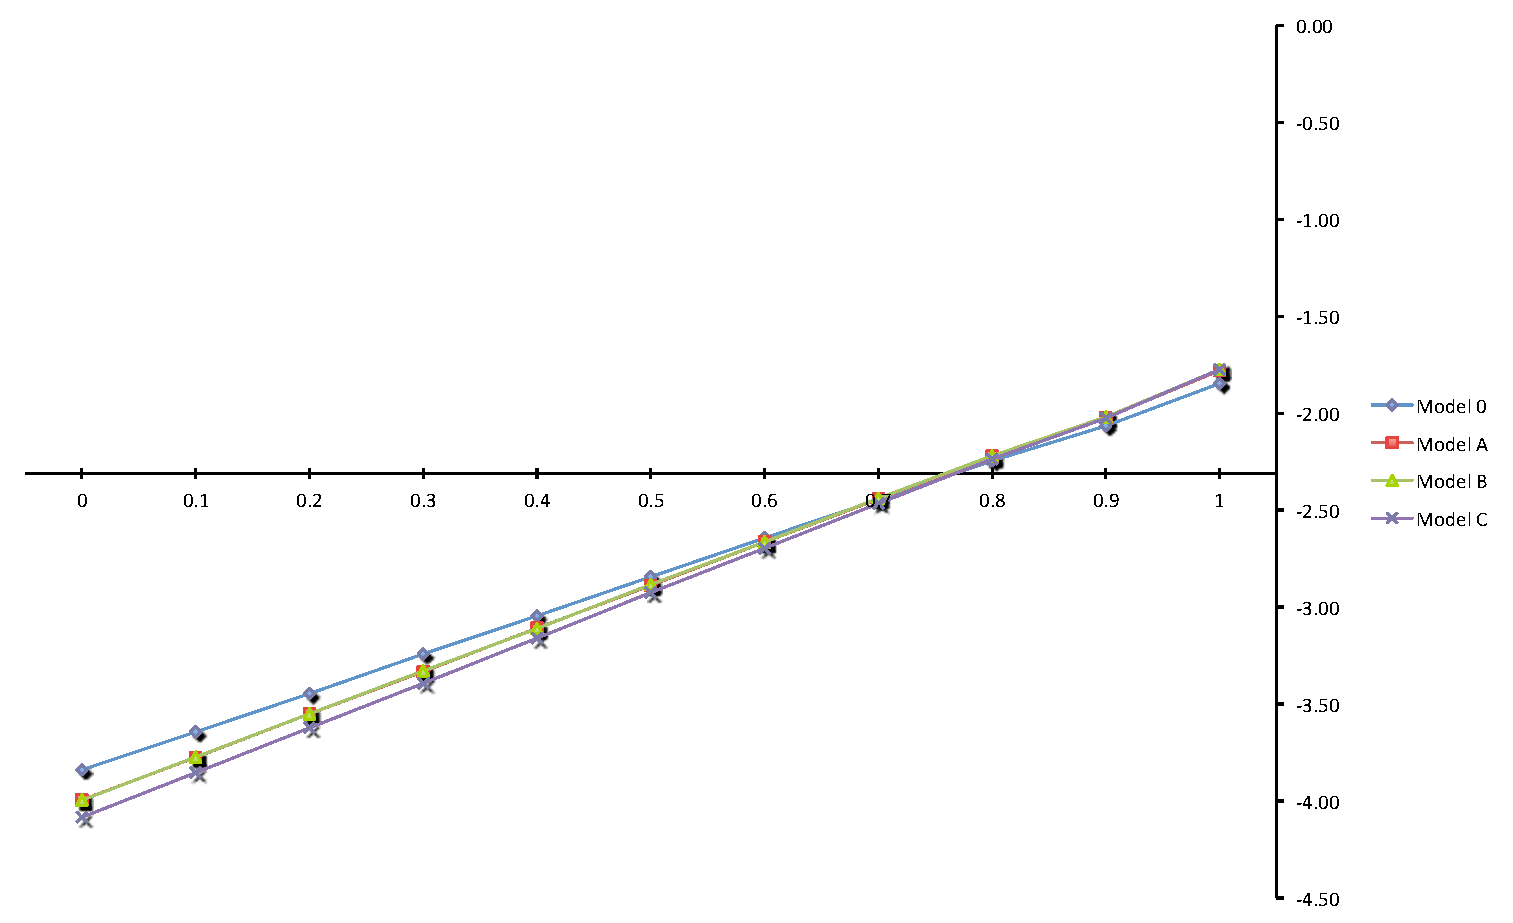
\includegraphics[width=8cm, height=5cm]{Case1.pdf}
\caption{Case 1}
\end{center}
\end{figure}

\subsubsection{Break in the trend under the alternative}

This set of results investigate the power of the test statistic when there is no unit root and no change in the intercept, $d\alpha_{i}=0$, but the trend dummy does change, $d\gamma_i=0.05$. When accommodating for both a trend and an intercept change (model C), the power of the test in rejecting the null of a unit root declines as the proportion of individuals with trend break increases. The power of the test is especially low in the case when nearly all individuals have a structural break. The results are similar when model A, modelling a level shift instead of a trend break, is used. However, the test statistics tend to be smaller in absolute value than with model C. Lastly, the test statistics are smaller than the two previous ones when the model does not accommodate for any type of break. These results have three implications (i) a break in trend can seriously affect the power of the proposed test even when the model is correctly specified. This is consistent with results in the time series literature; (ii) the power of the test depends on $c$, that is the porportion of individuals experience a break in trend; and (iii) although the power of the test is low even when the correct model is specified in this case, the test with the correct model still performs better than the misspecified model, this indicates the choice of model does matter.

\subsubsection{Break in the intercept under the alternative}
This batch of the simulation allows for a break in the intercept ($d\alpha_i=-0.5$) and no break in trend ($d\gamma_i=0$) while testing the null of a unit root. When the model accommodates for a break in trend rather than intercept (Model B), the test statistics have high power and reject the null even when a large proportion of the individuals experience a break in the intercept. These results seem to suggest that breaks in the intercepts do not have as much impact on the power of the test as breaks in the trend coefficients. Again, this is similar to the findings from time series literature for univariate time series.

\subsubsection{No breaks under the null}
If model C is selected, modelling both a trend and intercept break when there is no break, the test statistic does not reject the true null only when all individuals in the panel have a unit root. On the other hand, when the right model is chosen (that does not accommodate for any type of break), the test statistic does not rejects the true null if the proportion of individual that has a unit root is above $0.8$. Below that proportion, the tests rejects the null of a unit root while the DGP has one. The size of the test is not good, but it improves upon selection of the right model.

\begin{table} \label{table:cv}
\caption{Simulated critical values}
\begin{center}
\begin{tabular}{cccc}
\hline
Break Proportion&Case 4&Case 5&Case 6\\
\hline
0&-1.612&-1.663&-1.665\\
0.1&-1.645&-1.631&-1.646\\
0.2&-1.600&-1.656&-1.652\\
0.3&-1.590&-1.637&-1.654\\
0.4&-1.600&-1.648&-1.668\\
0.5&-1.618&-1.635&-1.644\\
0.6&-1.553&-1.650&-1.686\\
0.7&-1.643&-1.663&-1.620\\
0.8&-1.534&-1.643&-1.671\\
0.9&-1.632&-1.652&-1.634\\
1&-1.648&-1.638&-1.649\\
\hline
\end{tabular}
\end{center}
\end{table}%

\section{CONCLUSIONS}
This paper proposed a new unit root test for panel data accommodating unknown break-date by generalizing the testing procedure as proposed in \citet{KimPerron:2009}. Using the results in \citet{ChanManciniPauwels:2009}, the proposed test statistics is shown to be asymptotically normal. The test is then used to investigate the impact of model misspecification through Monte Carlo Simulations. The results suggested that the size and power of the test can be seriously distorted in the presence of a break in trend. However, breaks in the intercepts do not seem to affect the performance of the test seriously even when the incorrect model was chosen. Nevertheless, the overall results suggested that model misspecification does matter in testing for unit root in the presence of structural stability for panel data. Interestingly, most of the findings in this paper are consistent with the results for univariate time series.

\section*{Acknowledgement}
	The first author would like to thank the financial supports from the School of Economics and Finance, Curtin University of Technology. The second author would like to thank the financial supports from the Faculty of Economics and Business, Discipline of Econometrics and Business Statistics, University of Sydney. This paper was written while the second author was a visiting fellow at the School of Economics and Finance at the Curtin University of Technology, Perth, Australia. The hospitality of the school is gracefully acknowledged.

\bibliography{panelurootlit}
\bibliographystyle{chicago} %use chicago style of referencing.
\end{document}
